\chapter{Istniejące rozwiązania (Filip Korthals)}
\label{chap:example solutions}

W niniejszym rozdziale przedstawiono przykładowe rozwiązania zbliżone do problemu opisywanego w tej pracy.

\section{Aplikacja do planowania trasy drona - PIX4Dcapture}

PIX4Dcapture to aplikacja mobilna szwajcarskiej firmy Pix4D, udostępniająca mapy offline oraz planowanie trasy, które odbywa się za pomocą nanoszonych obszarów misji na mapę \cite{pix4dcapture}. Istnieje w niej także możliwość planowania siatki trasy oraz torów eliptycznych lub manualnego sterowania, aby przyjrzeć się danemu obiektowi. Na ich podstawie aplikacja wyznacza trasę dla drona przebiegającą po wybranym obszarze mającym z góry zdefiniowany tor ruchu. Głównym celem jest sfotografowanie całego terenu przez drona, aby następnie za pomocą innych narzędzi wykorzystać wykonane zdjęcia i dokonać mapowania terenu – w 2D lub 3D. Stosowane również jako przydatne narzędzie przy modelowaniu obiektów. Aplikacja jest dostępna na systemy Android i iOS, ale również na wybrane kontrolery do dronów. Co istotne, połączenie sieciowe nie jest wymagane podczas korzystania z aplikacji, więc nie ma problemu przy wykonywaniu przelotów w obszarach o słabym zasięgu sieci.

System oferowany przez Pix4D daje możliwość wybrania modelu drona, aby po zaplanowaniu trasy móc wgrać ją bezpośrednio do pamięci statku powietrznego. Aplikacja nie wspiera wszystkich dronów, kamer i kontrolerów, a ich lista jest określona w dokumentacji dostarczonej przez producenta \cite{pix4dcapture_supported}. Chcąc skonfigurować planowanie trasy, użytkownik jest proszony o wybór rodzaju misji. Każdy rodzaj ma inne zastosowanie i wyznacza, w jaki sposób dron będzie się przemieszczał po wybranym terenie. Najbardziej typowym rodzajem misji i sprawdzającym się w większości przypadków jest opcja \textit{Grid}, która tworzy trasę na kształt siatki w prostokątnym obszarze. Ma to zastosowanie przy mapowaniu dwuwymiarowym i tylko w przypadku pól prostokątnych. Do mapowania pól o nieregularnych kształtach została dodana opcja \textit{Polygon}, która umożliwia dostosowanie krawędzi nanoszonego obszaru do faktycznych granic pola. Następnie na wyznaczony obszar, podobnie jak w poprzednim przypadku, zostaje naniesiona siatka, po której ma poruszać się dron. Kolejnym rodzajem misji jest \textit{Double Grid}, który działa podobnie do zwykłego \textit{Grid}, przy czym na obszar nanoszone jest więcej siatek niż tylko jedna. Ma to na celu wykonanie zdjęć terenu z różnych stron, aby zebrać detale widoczne też w pionie, a nie tylko w poziomie. Takie podejście ma zastosowanie przy trójwymiarowym mapowaniu terenu. Z tego powodu, producent zaleca stosowanie tego trybu do latania w małej odległości od mapowanych obiektów \cite{pix4d_missions}. Następnym rodzajem misji jest misja \textit{Circular}, stworzona do dokładnego fotografowania obiektów ze wszystkich stron. Obszar należy umieścić tak, aby mapowany obiekt znajdował się w jego centrum. Dron podążający wyznaczoną trasą powinien obracać się równomiernie z zataczaniem okręgu wokół celu. W przypadku fotografowania obiektów wysokich – przykładowo wieżowców – producent zaleca wykonanie wielu takich misji na różnych wysokościach. Ostatni rodzaj misji nazywa się \textit{Free Flight} i został on stworzony do najbardziej skomplikowanych celów, do których nie pasuje żaden z uprzednio wymienionych trybów. W tym przypadku nie jest wyznaczana trasa, a pilot musi samodzielnie sterować dronem. Natomiast dzięki aplikacji PIX4Dcapture, zdjęcia są wykonywane automatycznie po przebyciu przez drona określonego dystansu – w pionie i poziomie.

\begin{figure}[H]
    \centering
    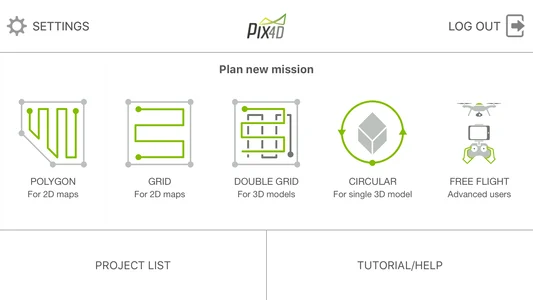
\includegraphics[width=\textwidth]{images/PIX4D_Wybor_misji.png}
    \caption{Wybór rodzaju misji}
\end{figure}

Parametry misji można dowolnie dostosowywać do własnych potrzeb. Można zarówno manipulować rozmiarem, jak i rotacją wybranego obszaru. Użytkownik ma możliwość dostosowania wysokości lotu oraz prędkości, z jaką dron ma się poruszać. Wybraną misję z konkretnymi ustawieniami można zapisać, aby wykorzystywać ją wielokrotnie w przyszłości.

\begin{figure}[H]
    \centering
    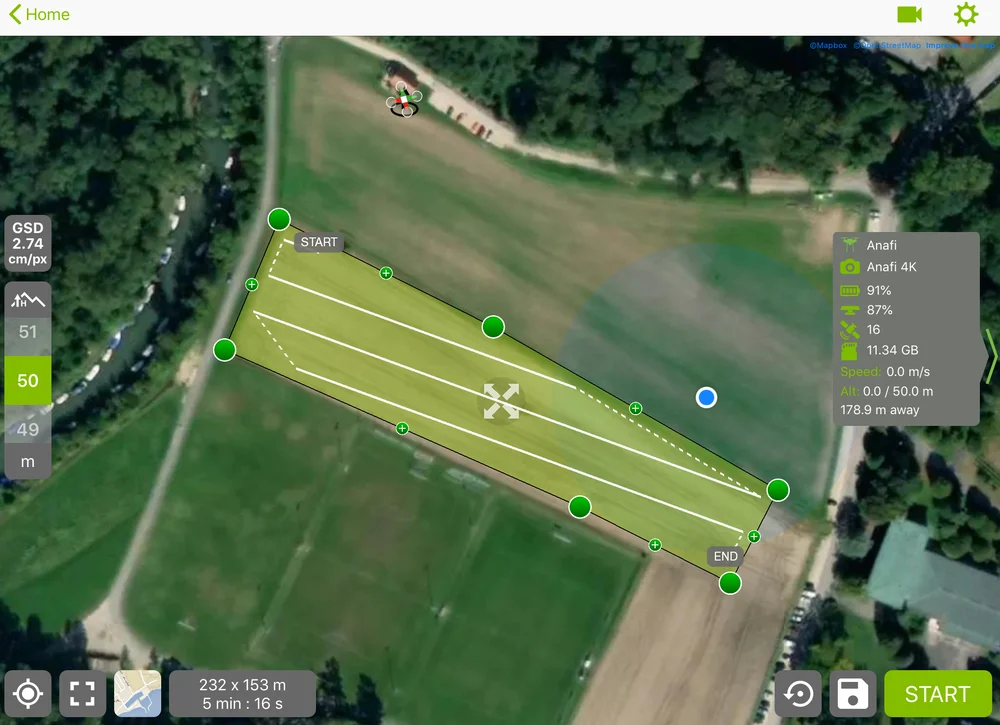
\includegraphics[width=\textwidth]{images/PIX4D_Przebieg_misji.png}
    \caption{Wybrana misja}
\end{figure}

Kolejnym krokiem jest już połączenie aplikacji z dronem i wgranie do pamięci urządzenia zaplanowanej trasy. Z poziomu aplikacji można wykonać start misji, po którym dron automatycznie wystartuje i wykona wgraną trasę. Zdjęcia również są wykonywane automatycznie, więc użytkownik musi jedynie kontrolować, czy wszystko przebiega zgodnie z planem. Po wykonanej misji dron sam wraca na miejsce startu. Wykonane fotografie można następnie przenieść do innych narzędzi służących do mapowania terenu, które producent również oferuje. Przy korzystaniu w tym celu z aplikacji od Pix4D, powstał format pliku .p4d, który bardzo ułatwia przenoszenie danych między aplikacjami i późniejszą pracę nad projektem.

Producent nie dostarcza zbyt wielu informacji na temat swojego produktu poza dokumentacją zawierającą dane o funkcjonalnościach systemu. Jest to przydatne narzędzie do planowania trasy, ale w konkretnym celu – w celu mapowania i modelowania. W przypadku problemu przedstawianego w niniejszej pracy, kiedy istotny jest aspekt skupienia się na konkretnym obszarze pola oraz najbardziej optymalnego wykorzystania baterii do pokrycia całego pola, aplikacja PIX4DCapture nie przynosiłaby zadowalających rezultatów.

\section{Aplikacja do kontroli lotu drona – Dronelink}

Dronelink to aplikacja umożliwiająca kontrolowanie lotu drona manualnie lub automatycznie i wyznaczanie trasy na mapie po z góry zdefiniowanym przez użytkownika obszarze. Pozwala ona też na pobieranie danych podczas lotu. Aplikacja jest dostępna zarówno w internecie, jak i na urządzenia mobilne oraz niektóre kontrolery do dronów. Jej celem jest pomoc przy fotografowaniu terenu lub obiektów w różnych celach – od hobbystycznych do profesjonalnych. Stąd grupą docelową produktu jest każdy użytkownik drona, który ma potrzebę realizowania precyzyjnych i powtarzalnych lotów.

Główną funkcjonalnością aplikacji jest planowanie trasy na podstawie nanoszenia szablonu \cite{dronelink}. Użytkownik jest proszony o wskazanie miejsca na mapie i naniesienie w dane miejsce szablonu dostarczonego przez producenta. Naniesiony wzór można dowolnie modyfikować pod swoje potrzeby. Możliwa jest ręczna konfiguracja rozmiaru pokrywanego obszaru, jego kształtu, kierunku planowanej trasy i miejsca startu czy lądowania drona. Aplikacja umożliwia również dostosowanie przebiegu trasy do ukształtowania terenu, co jest nietypowym rozwiązaniem w porównaniu do konkurencji. Przechodząc do kolejnych parametrów – użytkownikowi udostępniane są opcje modyfikacji już samego lotu – wysokość i prędkość przelotu czy kąt nachylenia kamery. To tylko część z oferowanych ustawień, ponieważ system ma ich wiele z racji na bardzo szeroki zakres możliwości jego wykorzystania. Po zapisaniu trasy, jest ona dostępna w bibliotece przypisanej do konta, więc można uzyskać do niej dostęp na każdym urządzeniu po zalogowaniu. Taką trasę można wgrać do pamięci statku powietrznego, który automatycznie wykona trasę. Dron jednak nie pozostaje jednak bez kontroli i pilot może w każdej chwili zatrzymać misję i przejąć kontrolę, w tym wywołać komendę powrotu drona na miejsce startu. Ma to zastosowanie choćby przy długich trasach. Drony często mają taką baterię, która nie pozwala na długi czas lotu. W takiej sytuacji pilot może przerwać misję, aby wymienić baterię i następnie wznowić lot. Aplikacja zapamiętuje miejsce, w którym została zatrzymana misja i po jej wznowieniu dron automatycznie wraca na miejsce przerwania, aby od tego miejsca zacząć dalsze fotografowanie według planu.

Wspomnianych szablonów producent zapewnia kilka podstawowych rodzajów, aby użytkownik mógł znaleźć wzór najbardziej dopasowany do swoich potrzeb. Pierwszym szablonem jest \textit{Map}, który jest przeznaczony do mapowania terenu. Działa na bardzo podobnej zasadzie jak w przypadku aplikacji PIX4Dcapture – na wyznaczony obszar nanoszona jest siatka, która umożliwi dronowi ujęcie kamerą całego oczekiwanego terenu. Kolejnym szablonem jest \textit{Waypoints}, który już nie ma na celu mapowania terenu, ale wyznaczenie ścieżki, którą ma przebyć dron, na podstawie naniesionych punktów orientacyjnych. Użytkownik może dowolnie dodawać i usuwać punkty, kształtować trasę między nimi lub konfigurować zachowanie drona na poszczególnych etapach lotu. Jest to wzorzec skierowany choćby do filmowców, aby uzyskać przelot, który będzie dokładnie spełniał wszystkie wymaganie i będzie przy tym mocno powtarzalny. Następnym szablonem, również istniejącym u konkurencji od firmy Pix4D, jest \textit{Circle}, który oferuje trasę krążenia wokół wybranego celu. To również może posłużyć do mapowania, ale już nie w poziomie, a w pionie – zwłaszcza konkretnych obiektów. Ostatnim oferowanym szablonem jest \textit{Pano}, które pozwala na utworzenie zdjęcia panoramicznego. Na podstawie zaplanowanej trasy dron wykonuje serię zdjęć, które następnie są łączone w jedno, spójne zdjęcie panoramiczne. Zdjęcie może być zarówno poziome, jak i pionowe. W aplikacji są dostępne jeszcze inne, zaawansowane szablony misji. Te trasy są już bardziej złożone i przeznaczone do bardziej specyficznych celów – raczej rzadko używane. Są to pewne konfiguracje tras podstawowych, ale na pewno daje to wygodę użytkownikowi, aby skorzystać ze złożonych szablonów zamiast ręcznie konfigurować szablon podstawowy.

Ciekawymi funkcjami przy planowaniu trasy są przegląd 3D oraz symulacja trasy. Przegląd 3D umożliwia obejrzenie zaplanowanej trasy ze wszystkich stron, a nie tylko w rzucie z góry przy standardowym patrzeniu na mapę. Pomaga to zobrazować zmiany w wysokościach lotu w poszczególnych momentach misji. Symulacja trasy natomiast pozwala sprawdzić przebieg całej trasy bardzo szczegółowo. Generowany jest wirtualny lot, w tym obraz na podstawie zdjęć satelitarnych z przewidywanym rezultatem, który może uzyskać dron. Są przy tym wyświetlane wszystkie parametry, takie jak: prędkość chwilowa, wysokość oraz przebyta droga. Dla jeszcze większej kontroli dodana jest oś czasu, która obrazuje co dokładnie się wydarzy w którym momencie lotu.

\begin{figure}[H]
    \centering
    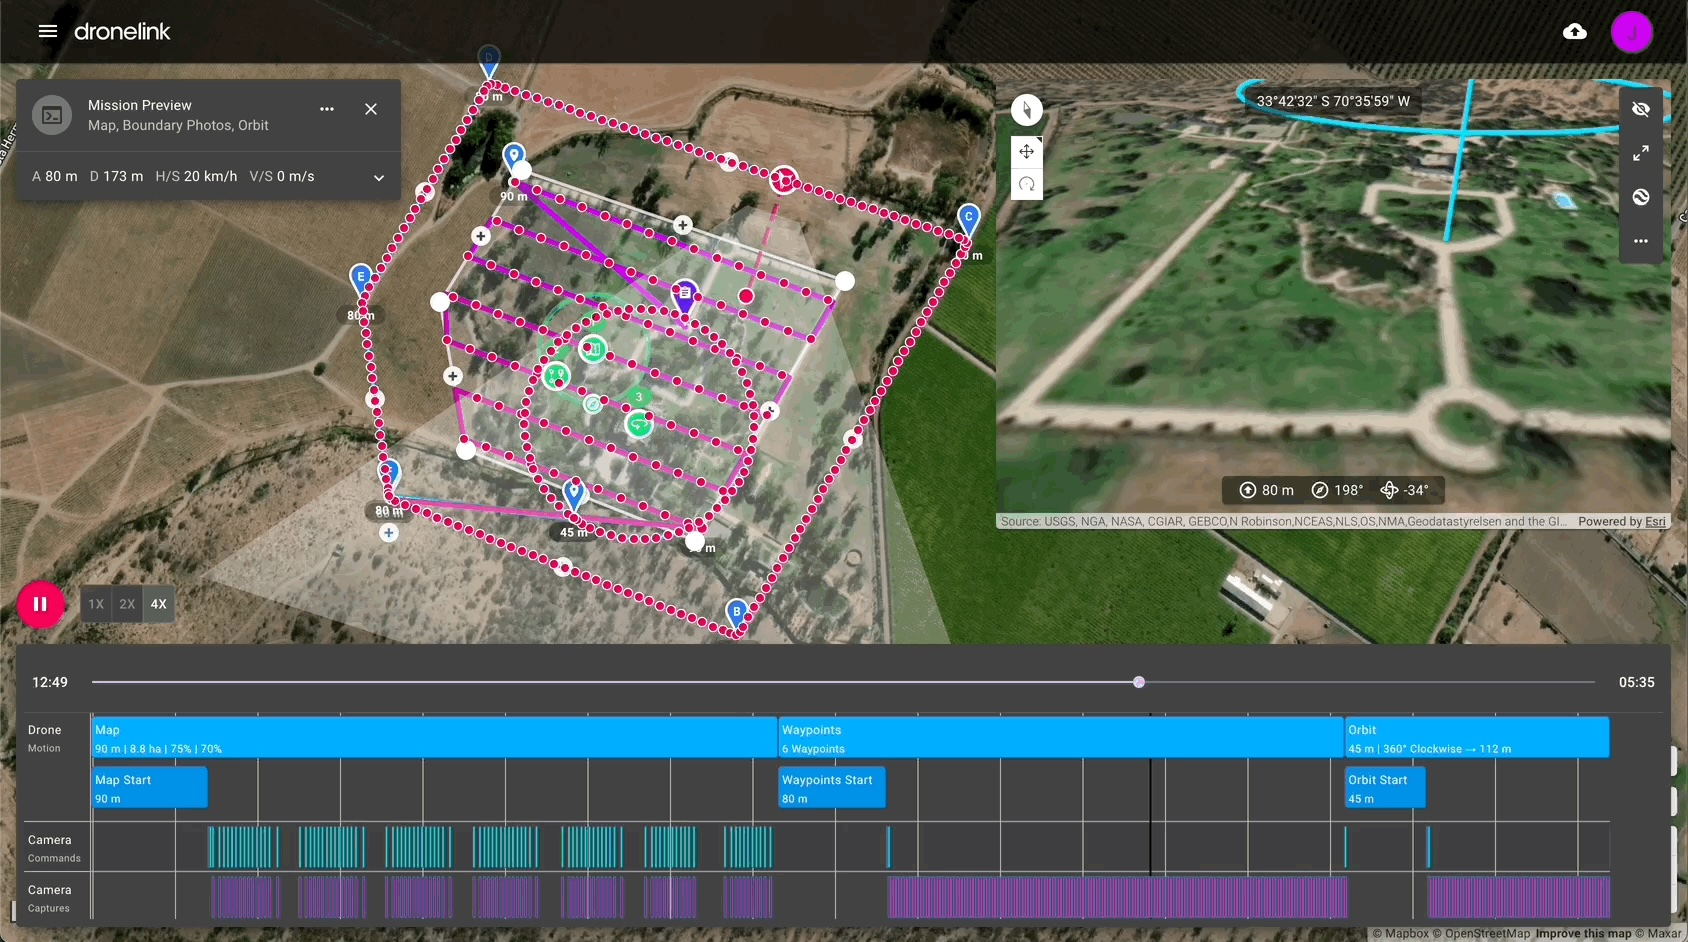
\includegraphics[width=\textwidth]{images/Dronelink_symulacja.jpg}
    \caption{Symulacja misji}
\end{figure}

Dronelink oferuje również inne tryby pracy, nie tylko planowanie tras z szablonów. Jednym z nich jest tryb misji \textit{On-the-fly}. Takie misje dają użytkownikowi wskazówki do wykonania konkretnych manewrów dronem, aby wytyczyć parametry do generowania trasy. Jednym typem takiej misji – bardziej opisanym przez producenta – jest \textit{On-the-fly Waypoints}. Polega on na wyznaczaniu punktów orientacyjnych za pomocą drona. Użytkownik łączy drona z aplikacją i ręcznie wykonuje lot. Następnie w aplikacji zaznacza miejsca, w których dron się akurat znajduje. W ten sposób użytkownik sam wybiera punkty, na których mu zależy. Dzięki temu, punkty mogą być wskazane na podstawie faktycznego widoku z kamery, a nie tylko położenia na mapie, które może być niewystarczającym wyznacznikiem położenia oczekiwanego kadru. W dalszej fazie z wyznaczonych punktów orientacyjnych zostaje wytyczona trasa, którą można modyfikować tak samo, jak w przypadku trasy z szablonu.

\begin{figure}[H]
    \centering
    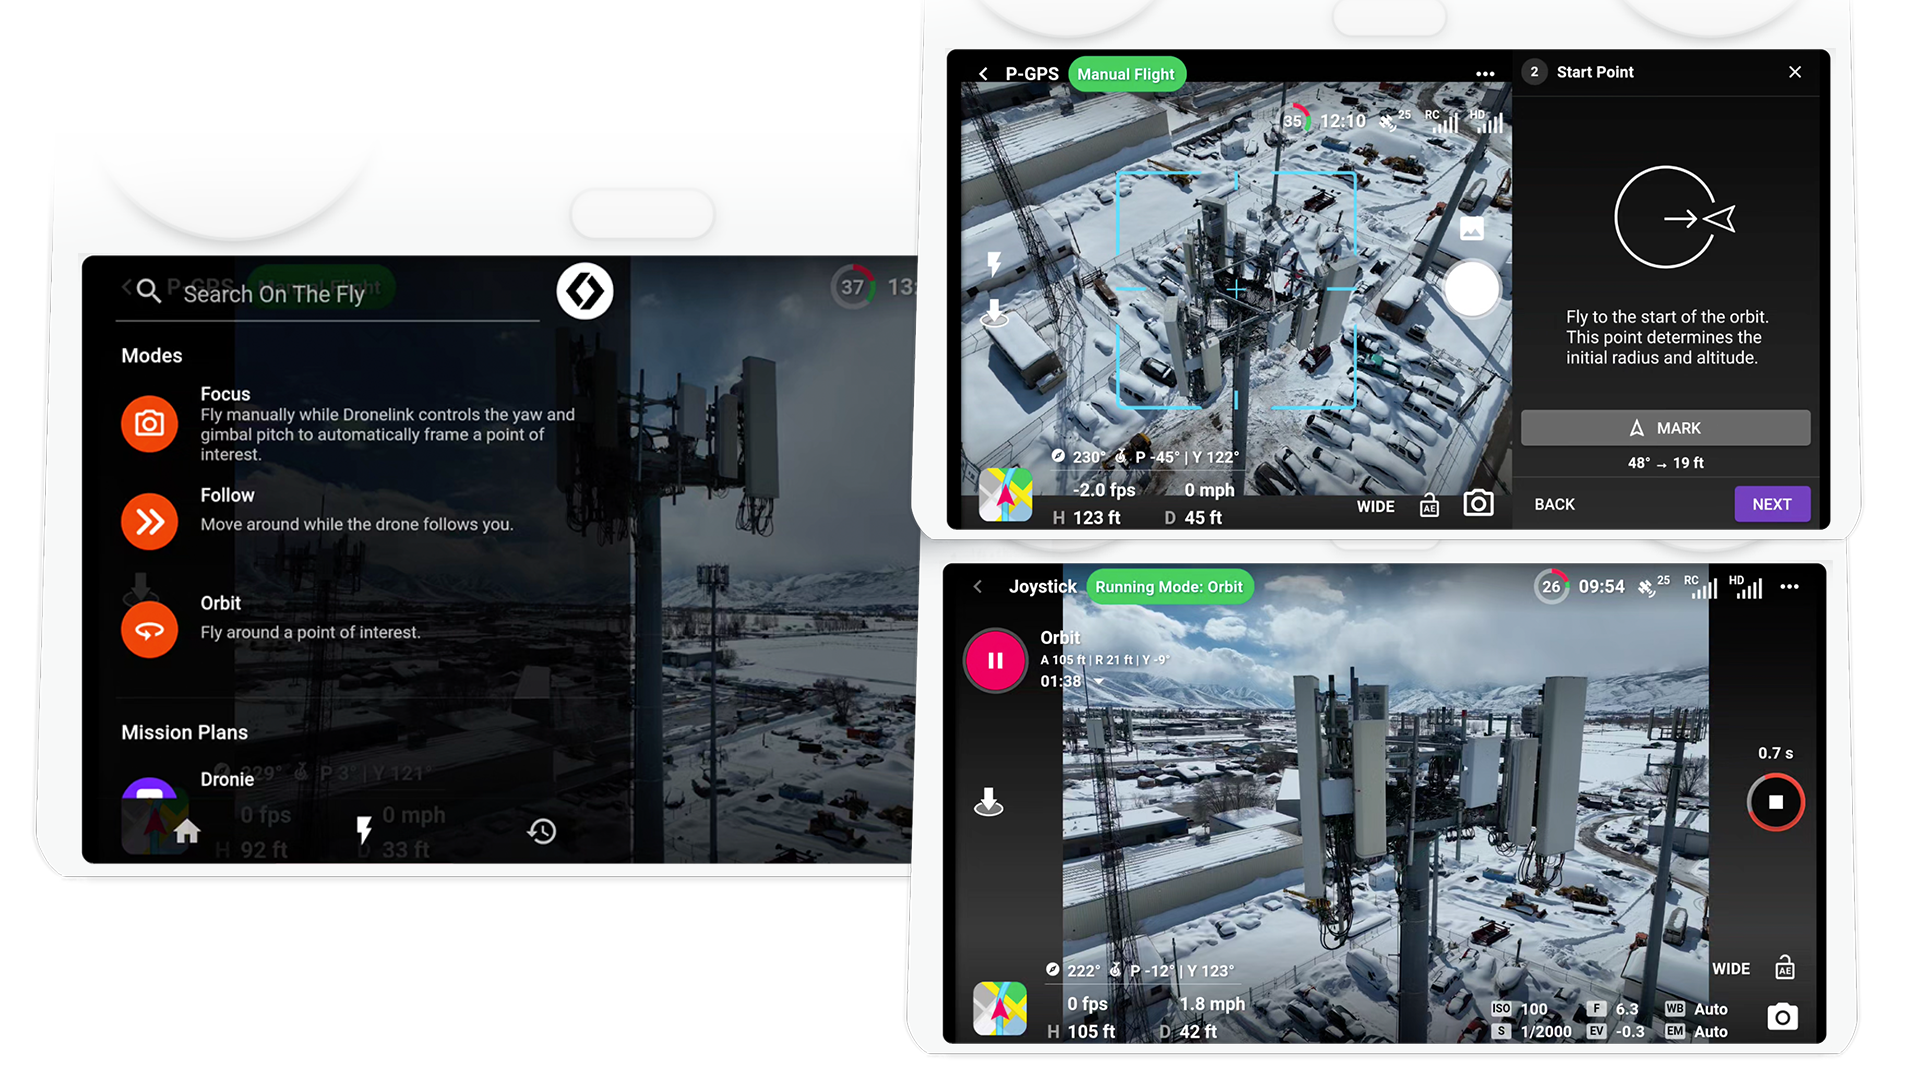
\includegraphics[width=\textwidth]{images/Dronelink_misje_hybrydowe.png}
    \caption{Przegląd misji hybrydowych}
\end{figure}

Trzeci i ostatni tryb pracy determinuje tryb lotu drona. Są to misje hybrydowe, czyli część działań jest wykonywana automatycznie, a część jest pozostawiona kontroli użytkownika. W ten sposób użytkownik ma kontrolę nad działaniami drona, ale ta praca jest uproszczona, więc można się skupić na tym, na czym najbardziej użytkownikowi zależy. W tym trybie oferowane są trzy rodzaje lotów: \textit{Focus}, \textit{Follow} i \textit{Orbit}. Pierwszy z wymienionych daje użytkownikowi swobodę w sterowaniu dronem, ale pomaga przy ujęciach wybranego celu. Wymagane do tego jest ustawienie celu, którego użytkownik chce wykonać zdjęcia. Następnie, podczas lotu, dron automatycznie będzie się obracał i kierował kamerę na wybrany wcześniej cel. Użytkownik może dynamicznie dobierać miejsce, z którego ma być wykonane ujęcie, bez jednoczesnego zajmowania się ustawianiem kamery. Drugi rodzaj lotu z wymienionych, czyli \textit{Follow}, wprowadza funkcję śledzenia użytkownika. Dron na bieżąco podąża za urządzeniem z aplikacją Dronelink oraz dostosowuje kamerę tak, aby cel znajdował się w centrum. Istnieje przy tym kilka opcji dostosowania parametrów lotu do swoich potrzeb. Są to: ustawienia korzystania z kontrolera do korekcji położenia drona, ustawienie dynamicznego punktu lądowania – aby dron wrócił do użytkownika zamiast do miejsca startu, automatyczne dostosowywanie wysokości lotu do ukształtowania terenu oraz automatyczny start nagrywania. Ostatni rodzaj lotu – \textit{Orbit} – łączy cechy misji \textit{Circle} oraz \textit{Focus}. Użytkownik jest proszony o wyznaczenie punktów określających obiekt, który ma być fotografowany. Następnie, po podaniu wszystkich wymaganych parametrów, generowana jest trasa, według której dron orbituje wokół obiektu. Użytkownik w trakcie lotu ma pełną kontrolę nad dronem i może za pomocą kontrolera na bieżąco modyfikować lot. 

Aplikacja Dronelink oferuje opcję integracji z innymi systemami w celu wygodniejszej pracy nad uzyskanymi danymi. Producent na swojej stronie opisuje współpracę swojego produktu z systemami WebODM, Airdata oraz Pix4D. W przypadku dwóch ostatnich, aplikacja umożliwia bezpośrednie połączenie systemów w celu szybszego i łatwiejszego przesyłania danych.

Opisywany system jest dostępny na przeglądarki internetowe, niektóre kontrolery oraz urządzenia mobilne z systemem Android i iOS tworząc w ten sposób wysoką dostępność produktu dla użytkownika. Zakres obsługiwanych dronów jest już bardziej ograniczony. Pełna lista jest dostępna na stronie producenta \cite{dronelink_supported}. Są to w większości urządzenia producenta DJI. Jest to popularna marka dronów, ale wciąż dla posiadaczy urządzeń od innych producentów stanowi to jakieś ograniczenie. Natomiast od strony wsparcia technicznego, producent udostępnia stronę internetową z licznymi poradnikami. Są wśród nich instrukcje używania poszczególnych funkcjonalności, w tym nagrania wideo z komentarzem. Niestety producent nie dostarcza żadnej dokumentacji technicznej do produktu. Niektóre komponenty są opisane jedynie powierzchownie, a poradniki dotyczą tylko wybranych elementów. Nawet dosyć szczegółowe poradniki nie opisują dokładnie każdego elementu, a jedynie podstawowy sposób użycia danej funkcjonalności. Z tego powodu trudno jest dotrzeć do wszystkich szczegółów na temat aplikacji bez jej zakupu.

Dronelink jest produktem płatnym, dostępnym w planach subskrypcyjnych lub płatnych jednorazowo. Pojedynczy zakup dotyczy planów hobbystycznych – do celów rekreacyjnych, edukacyjnych i non-profit. W ofercie są trzy takie plany. Najtańszy jest plan podstawowy, a pozostałe – odpowiednio droższe – stanowią kolejne rozszerzenia tego planu. Analogicznie sytuacja się prezentuje w przypadku subskrypcji. Plany te są skierowane do celów profesjonalnych, komercyjnych. Zawierają one już bardzo zaawansowane narzędzia, dodatkowe opcje dostosowania oprogramowania do własnych potrzeb oraz zapewnione wsparcie producenta. Plany subskrypcyjne umożliwiają rozliczenie roczne lub miesięczne. Dzięki tak wielu opcjom zakupu dostępu do produktu użytkownik może wybrać plan najbardziej zbliżony do swoich potrzeb bez konieczności przepłacania za nadmiarowe funkcje, z których nie skorzysta.